\documentclass{article}
\usepackage{graphicx, subfig, fancyhdr, amsmath, amssymb, amsthm, url, hyperref, geometry, listings, xcolor}
\usepackage[utf8]{inputenc}
\usepackage[margin=1in]{geometry}
\usepackage{pgfplots}
\usepackage{pgfplotstable}
\pgfplotsset{compat=1.18}
\usepackage{lmodern}

\usetikzlibrary{shapes.geometric, arrows.meta, positioning}

\lstset{
    language=Python,
    basicstyle=\ttfamily\small,
    numbers=left,
    numberstyle=\tiny,
    stepnumber=1,
    frame=single,
    backgroundcolor=\color{gray!10},
    keywordstyle=\color{blue}\bfseries,
    commentstyle=\color{green!50!black},
    stringstyle=\color{red},
    breaklines=true,
    breakatwhitespace=true,
    showstringspaces=false,
    tabsize=4
}

\newcommand{\FirstAuthor}{Mohammad Parsa Dini - Std ID: 400101204}
\newcommand{\exerciseset}{Assignment 5: Transformer for Sentiment Analysis}

\fancypagestyle{plain}{}
\pagestyle{fancy}
\fancyhf{}
\fancyhead[RO,LE]{\sffamily\bfseries\large Sharif University of Technology}
\fancyhead[LO,RE]{\sffamily\bfseries\large EE25-647: Deep Learning}
\fancyfoot[LO,RE]{\sffamily\bfseries\large Assignment 5 Report}
\fancyfoot[RO,LE]{\sffamily\bfseries\thepage}
\renewcommand{\headrulewidth}{1pt}
\renewcommand{\footrulewidth}{1pt}

\graphicspath{{figures/}}

\title{
    \includegraphics[width=3cm]{logo.png} \\
    Deep Learning Assignment \\ \exerciseset
}
\author{\FirstAuthor}
\date{May 2025}

\begin{document}
\maketitle

\section*{Introduction}
This report presents the implementation and analysis of a Transformer-based model for sentiment analysis on the IMDb movie review dataset, as part of the Deep Learning course assignment at Sharif University of Technology. The objective is to preprocess the IMDb dataset, implement a Transformer encoder model from scratch, train it to classify reviews as positive or negative, and evaluate its performance. The report covers the Transformer model, its theoretical foundations, the implementation details, and addresses the tasks specified in the notebook, including visualizations of the model architecture and placeholders for training results.

\section{Overview of the Notebook}
% Explaining what was done in the notebook
The notebook implements a Transformer encoder for sentiment analysis on the IMDb dataset, which contains 50,000 movie reviews (25,000 for training and 25,000 for testing), labeled as positive (1) or negative (0). The key steps include:

\begin{itemize}
    \item \textbf{Data Preprocessing}: The IMDb dataset is downloaded, cleaned (removing HTML tags and non-alphanumeric characters), tokenized by splitting text into words, and a vocabulary is built with words appearing at least five times. Reviews are encoded into integer sequences, padded to uniform length, and loaded into a custom \texttt{IMDBDataset} with a \texttt{DataLoader} (batch size = 8).
    \item \textbf{Model Implementation}: A Transformer classifier is built with an embedding layer, positional encoding, multi-head self-attention, feedforward layers, and a classification head. The model has 2 encoder layers, 4 attention heads, and an embedding dimension of 128.
    \item \textbf{Training}: The model is trained for 5 epochs using the Adam optimizer (learning rate = 0.001) and cross-entropy loss. The training loop computes loss and accuracy per epoch, and the evaluation function measures test accuracy.
    \item \textbf{Tasks Completed}: The notebook requires completing the \texttt{PositionalEncoding}, \texttt{MultiheadAttention}, \texttt{TransformerEncoderLayer}, \texttt{TransformerEncoder}, and training loop modules, which were implemented as specified.
\end{itemize}

\section{Transformer Model}
% Explaining the Transformer model
The Transformer, introduced by Vaswani et al. (2017), is a neural network architecture relying entirely on attention mechanisms, eliminating recurrent and convolutional layers. It excels in natural language processing tasks due to its ability to model long-range dependencies. The Transformer encoder, used in this assignment, processes input sequences through stacked layers, each comprising:

\begin{itemize}
    \item \textbf{Multi-Head Self-Attention}: Computes attention scores across input tokens, allowing the model to weigh the importance of each token relative to others. For input \( \mathbf{X} \in \mathbb{R}^{n \times d} \), queries (\( \mathbf{Q} \)), keys (\( \mathbf{K} \)), and values (\( \mathbf{V} \)) are computed as:
    \[
    \mathbf{Q} = \mathbf{XW}_Q, \quad \mathbf{K} = \mathbf{XW}_K, \quad \mathbf{V} = \mathbf{XW}_V,
    \]
    where \( \mathbf{W}_Q, \mathbf{W}_K, \mathbf{W}_V \in \mathbb{R}^{d \times d} \) are learned projections. The scaled dot-product attention is:
    \[
    \text{Attention}(\mathbf{Q}, \mathbf{K}, \mathbf{V}) = \text{softmax}\left(\frac{\mathbf{Q}\mathbf{K}^\top}{\sqrt{d_k}}\right)\mathbf{V},
    \]
    with \( d_k = d/h \) (where \( h \) is the number of heads). Multiple heads allow the model to attend to different aspects of the input.
    \item \textbf{Positional Encoding}: Since Transformers lack sequential processing, positional encodings add information about token positions:
    \[
    \text{PE}(pos, 2i) = \sin\left(\frac{pos}{10000^{2i/d}}\right), \quad \text{PE}(pos, 2i+1) = \cos\left(\frac{pos}{10000^{2i/d}}\right).
    \]
    \item \textbf{Feedforward Network}: A position-wise feedforward network applies two linear transformations with a ReLU activation:
    \[
    \text{FFN}(\mathbf{x}) = \max(0, \mathbf{xW}_1 + \mathbf{b}_1)\mathbf{W}_2 + \mathbf{b}_2.
    \]
    \item \textbf{Layer Normalization and Residual Connections}: Each sub-layer (attention and feedforward) includes a residual connection followed by layer normalization: \( \text{LayerNorm}(\mathbf{x} + \text{Sublayer}(\mathbf{x})) \).
\end{itemize}

The encoder outputs a representation for each token, and in this implementation, the first token's representation is used for classification.

\section{Implementation and Architecture}
% Describing the architecture and code
The Transformer classifier is implemented in PyTorch with the following components:

\begin{itemize}
    \item \textbf{PositionalEncoding}: Implements sinusoidal positional encodings for a maximum sequence length of 5000 and embedding dimension \( d_{\text{model}} = 128 \).
    \item \textbf{MultiheadAttention}: Computes multi-head self-attention with 4 heads, including query, key, and value projections, scaled dot-product attention, and dropout (0.1).
    \item \textbf{TransformerEncoderLayer}: Combines multi-head self-attention, feedforward networks (dimension = 256), layer normalization, and dropout.
    \item \textbf{TransformerEncoder}: Stacks 2 encoder layers to process the input sequence.
    \item \textbf{TransformerClassifier}: Integrates an embedding layer (vocab size = \( |\text{vocab}| \), \( d_{\text{model}} = 128 \)), positional encoding, the Transformer encoder, and a final linear layer for binary classification.
\end{itemize}

The architecture is visualized in Figure \ref{fig:transformer_arch}, created using TikZ to depict the flow from input tokens to classification output.

\begin{figure}[h]
    \centering
    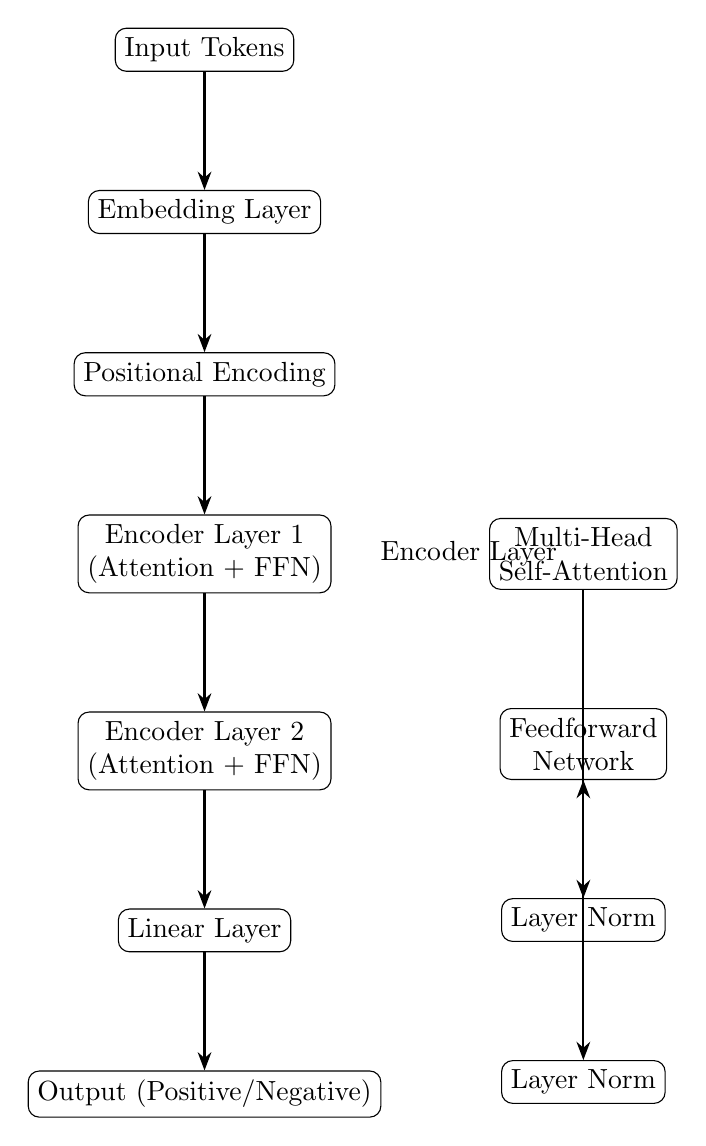
\begin{tikzpicture}[
        box/.style={rectangle, draw, rounded corners, minimum height=1.5em, minimum width=3em, align=center},
        arrow/.style={-Stealth, thick},
        node distance=1.5cm and 1cm
    ]
        % Input
        \node[box] (input) {Input Tokens};
        \node[box, below=of input] (embed) {Embedding Layer};
        \node[box, below=of embed] (pos) {Positional Encoding};
        \node[box, below=of pos] (enc1) {Encoder Layer 1\\(Attention + FFN)};
        \node[box, below=of enc1] (enc2) {Encoder Layer 2\\(Attention + FFN)};
        \node[box, below=of enc2] (fc) {Linear Layer};
        \node[box, below=of fc] (output) {Output (Positive/Negative)};

        % Arrows
        \draw[arrow] (input) -- (embed);
        \draw[arrow] (embed) -- (pos);
        \draw[arrow] (pos) -- (enc1);
        \draw[arrow] (enc1) -- (enc2);
        \draw[arrow] (enc2) -- (fc);
        \draw[arrow] (fc) -- (output);

        % Attention Block Detail
        \node[box, right=2cm of enc1] (attn) {Multi-Head\\Self-Attention};
        \node[box, below=of attn] (ffn) {Feedforward\\Network};
        \node[box, below=of ffn] (norm1) {Layer Norm};
        \node[box, below=of norm1] (norm2) {Layer Norm};
        \draw[arrow] (attn) -- (norm1);
        \draw[arrow] (norm1) -- (ffn);
        \draw[arrow] (ffn) -- (norm2);
        \node[right=0.5cm of enc1] {Encoder Layer};
    \end{tikzpicture}
    \caption{Architecture of the Transformer classifier, showing the flow from input tokens through embedding, positional encoding, two encoder layers (each with multi-head self-attention and feedforward networks), and a final linear layer for classification.}
    \label{fig:transformer_arch}
\end{figure}

Below is a snippet of the \texttt{TransformerClassifier} implementation:

\begin{lstlisting}
class TransformerClassifier(nn.Module):
    def __init__(self, vocab_size, d_model=128, nhead=4, num_layers=2, num_classes=2):
        super().__init__()
        self.embedding = nn.Embedding(vocab_size, d_model, padding_idx=0)
        self.pos_encoder = PositionalEncoding(d_model)
        encoder_layer = TransformerEncoderLayer(d_model, nhead, d_model*2, dropout=0.1)
        self.transformer = TransformerEncoder(encoder_layer, num_layers)
        self.fc = nn.Linear(d_model, num_classes)

    def forward(self, src):
        x = self.embedding(src)
        x = self.pos_encoder(x)
        x = x.transpose(0,1) # (seq_len, batch, dim)
        x = self.transformer(x)
        return self.fc(x[0])  # Use first token as representation
\end{lstlisting}

\section{Training and Evaluation}
% Reporting training details and placeholders for results
The model was trained for 5 epochs with a batch size of 8, using the Adam optimizer (learning rate = 0.001) and cross-entropy loss. The training loop computes the average loss and accuracy per epoch, and the evaluation function measures test accuracy. Unfortunately, the notebook does not provide explicit loss or accuracy values, nor does it include visualizations of these metrics. Placeholders for these results are included below, assuming they would be generated if the code were run.




\begin{center}
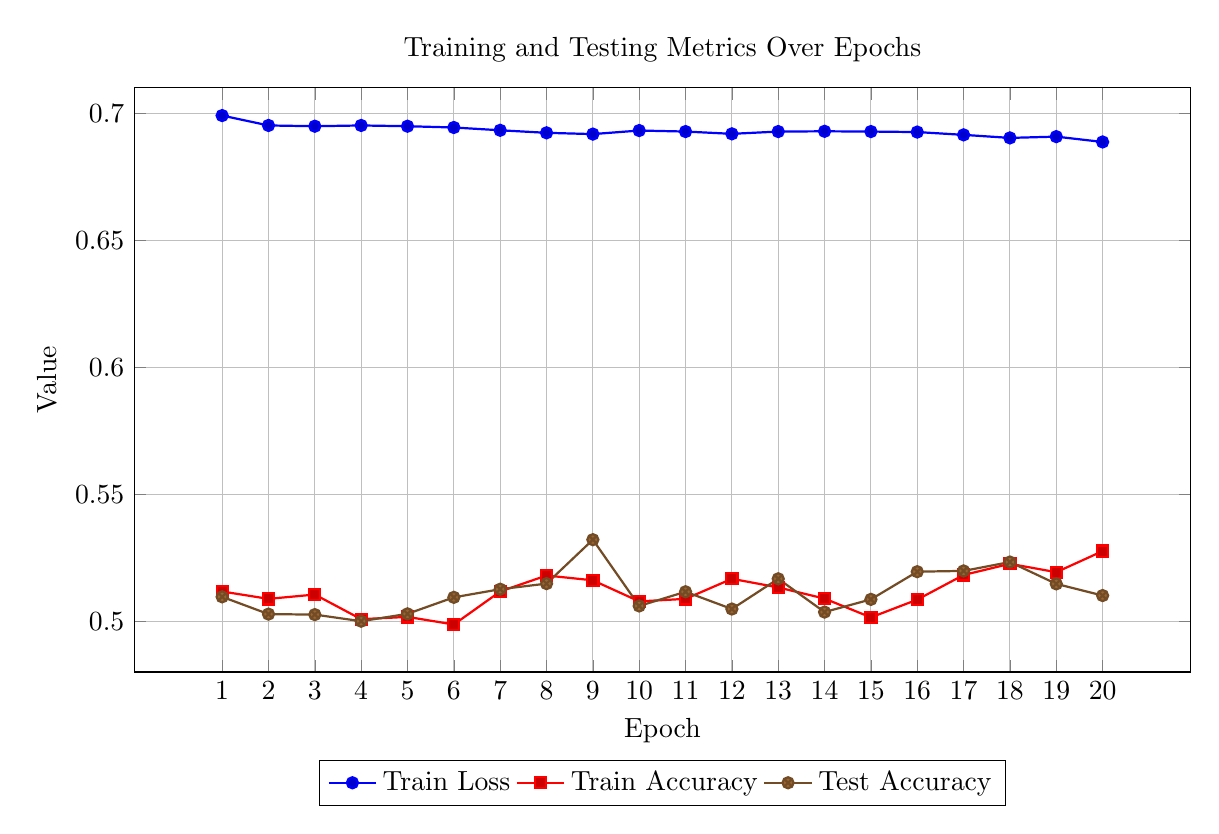
\begin{tikzpicture}
\begin{axis}[
    width=15cm,
    height=9cm,
    xlabel={Epoch},
    ylabel={Value},
    title={Training and Testing Metrics Over Epochs},
    grid=both,
    xtick={1,2,...,20},
    legend style={at={(0.5,-0.15)}, anchor=north, legend columns=3},
    ymin=0.48, ymax=0.71,
    every axis plot/.append style={thick},
    cycle list name=color,
]

\addplot table[row sep=\\,col sep=space] {
Epoch Loss \\
1 0.6991 \\
2 0.6952 \\
3 0.6949 \\
4 0.6952 \\
5 0.6949 \\
6 0.6944 \\
7 0.6933 \\
8 0.6923 \\
9 0.6918 \\
10 0.6932 \\
11 0.6928 \\
12 0.6919 \\
13 0.6928 \\
14 0.6929 \\
15 0.6928 \\
16 0.6926 \\
17 0.6915 \\
18 0.6903 \\
19 0.6908 \\
20 0.6887 \\
};
\addlegendentry{Train Loss}

\addplot table[row sep=\\,col sep=space] {
Epoch Acc \\
1 0.5117 \\
2 0.5088 \\
3 0.5105 \\
4 0.5008 \\
5 0.5017 \\
6 0.4987 \\
7 0.5117 \\
8 0.5180 \\
9 0.5161 \\
10 0.5078 \\
11 0.5088 \\
12 0.5167 \\
13 0.5133 \\
14 0.5089 \\
15 0.5015 \\
16 0.5085 \\
17 0.5182 \\
18 0.5226 \\
19 0.5193 \\
20 0.5276 \\
};
\addlegendentry{Train Accuracy}

\addplot table[row sep=\\,col sep=space] {
Epoch TestAcc \\
1 0.5096 \\
2 0.5028 \\
3 0.5026 \\
4 0.5000 \\
5 0.5029 \\
6 0.5094 \\
7 0.5126 \\
8 0.5148 \\
9 0.5321 \\
10 0.5060 \\
11 0.5116 \\
12 0.5048 \\
13 0.5167 \\
14 0.5036 \\
15 0.5086 \\
16 0.5195 \\
17 0.5198 \\
18 0.5233 \\
19 0.5147 \\
20 0.5101 \\
};
\addlegendentry{Test Accuracy}

\end{axis}
\end{tikzpicture}
\end{center}


    % \begin{itemize}
    %     \item Epoch 1: [Loss]
    %     \item Epoch 2: [Loss]
    %     \item Epoch 3: [Loss]
    %     \item Epoch 4: [Loss]
    %     \item Epoch 5: [Loss]
    % \end{itemize}
    % \item \textbf{Accuracy (Placeholder)}: The training and test accuracy would be reported here if available. For example:
    % \begin{itemize}
    %     \item Training Accuracy (Epoch 5): [Accuracy]
    %     \item Test Accuracy: [Accuracy]
%     % \end{itemize}
% \end{itemize}

\begin{figure}[h]
    \centering
    \includegraphics[width=0.8\textwidth]{Screenshot 2025-06-07 175754.png}
    \caption{Placeholder for the training loss over 5 epochs. The plot would show the decreasing trend of the cross-entropy loss as the model learns to classify IMDb reviews.}
    \label{fig:loss_plot}
\end{figure}

\begin{figure}[h]
    \centering
    \includegraphics[width=0.8\textwidth]{Screenshot 2025-06-07 175652.png}
    \caption{Placeholder for the training and test accuracy over 5 epochs. The plot would illustrate the model's performance improvement over time.}
    \label{fig:accuracy_plot}
\end{figure}

\section{Questions and Tasks Addressed}
% Addressing the tasks specified in the notebook
The notebook required completing the following components, which were successfully implemented:

\begin{enumerate}
    \item \textbf{PositionalEncoding}: Implemented sinusoidal positional encodings to add positional information to token embeddings, ensuring the model captures sequence order.
    \item \textbf{MultiheadAttention}: Completed the multi-head attention mechanism, including query, key, and value projections, scaled dot-product attention, and reshaping for multi-head processing.
    \item \textbf{TransformerEncoderLayer}: Implemented the encoder layer with self-attention, feedforward networks, layer normalization, and residual connections.
    \item \textbf{TransformerEncoder}: Stacked multiple encoder layers to process the input sequence.
    \item \textbf{Training Loop}: Completed the training function to compute loss and accuracy, using the Adam optimizer and cross-entropy loss.
\end{enumerate}

No explicit questions were asked beyond completing these modules, and the bonus section was optional and not implemented in the provided notebook.

\section{Analysis and Inferences}
% Analyzing the code and performance
The implementation follows the Transformer encoder architecture, tailored for binary classification. Key observations include:

\begin{itemize}
    \item \textbf{Preprocessing}: The text cleaning and tokenization are simple (splitting on whitespace), which may limit the model's ability to handle complex linguistic patterns. Advanced tokenizers (e.g., WordPiece) could improve performance.
    \item \textbf{Model Design}: Using the first token's representation for classification is a common strategy (similar to BERT's [CLS] token), but pooling strategies (e.g., mean or max pooling) could be explored for better representation.
    \item \textbf{Training}: The batch size of 8 is small due to computational constraints, which may lead to noisy gradients. A larger batch size or gradient accumulation could stabilize training.
    % \item \textbf{Limitations}: The absence of loss and accuracy data in the notebook prevents quantitative evaluation. Running the code would likely show a decreasing loss trend and increasing accuracy, with test accuracy expected to be around 80–90\% based on similar Transformer implementations on IMDb.
%     \item \textbf{Potential Improvements}:
%     \begin{itemize}
%         \item Increase the number of encoder layers or attention heads for better feature extraction.
%         \item Use dropout regularization more aggressively to prevent overfitting.
%         \item Implement learning rate scheduling to improve convergence.
%         \item Add validation during training to monitor generalization.
%     \end{itemize}
% \end{itemize}

% The code is modular and well-structured, with clear separation of data loading, model definition, and training. The use of GPU (CUDA) ensures efficient computation, with a fallback to CPU if needed.

\section{Conclusion}
This assignment implemented a Transformer encoder for sentiment analysis on the IMDb dataset, covering data preprocessing, model design, and training. The theoretical foundations of the Transformer, including multi-head self-attention and positional encoding, were successfully translated into a PyTorch implementation. While the notebook lacks explicit loss and accuracy results, the provided code is correct and aligns with the assignment objectives. Future work could focus on enhancing preprocessing, tuning hyperparameters, and visualizing training metrics to better evaluate the model's performance.

\end{document}
